\newpage
\section{Hypothesis Testing}
In this section, we study another central topic in statistics: Hypothesis Testing. The section is organized as follows: 
\begin{enumerate}
    \item Fundamentals
    \item Multiple Testing and Error Rate Control
    \item Causal Inference
    \item Conformal Prediction
    \item Watermark Detection
\end{enumerate}

This section mainly follows STAT300A (Stanford University), STAT300C (Stanford University), STATS361 (Stanford University) and Mathematics Statistics (Peking University, taught by Fang Yao).

\subsection{Fundamentals}
Hypothesis testing is just a particular type of decision problem. As usual, we 
assume that the data is sampled according to $X \sim \mathbb{P}_\theta$ and that 
$\mathbb{P}_\theta$ belongs to the model 
$\mathcal{P} = \{\mathbb{P}_\theta : \theta \in \Omega\}$. In addition to the 
standard setup, we divide the models in $\mathcal{P}$ into two disjoint subclasses 
known as ``hypotheses'':
\[
  \begin{aligned}
    H_0 &: \theta \in \Omega_0 \subset \Omega && \text{(null hypothesis)} \\
    H_1 &: \theta \in \Omega_1 = \Omega \setminus \Omega_0 && \text{(alternative hypothesis)}
  \end{aligned}
\]

Our goal is to infer which hypothesis is correct. This can be cast as classification, 
so our decision space is
\[
  \mathcal{D} = \{\text{accept } H_0,\ \text{reject } H_0\}.
\]

\begin{table}[h]
  \centering
  \begin{tabular}{r|l|l|}
    \cline{2-3}
                                  & $\theta \in \Omega_0$  & $\theta \in \Omega_1$   \\ \hline
    \multicolumn{1}{|r|}{Reject $H_0$} & 1 (Type I Error)       & 0 (Good)                \\ \hline
    \multicolumn{1}{|r|}{Accept $H_0$} & 0 (Good)               & 1 (Type II Error)       \\ \hline
  \end{tabular}
  \caption{Canonical loss function $L(\theta, d)$.}
  \label{tab:canonical-loss}
\end{table}

We have two types of error which induce a loss. A Type I error or false positive occurs when we reject $H_0$ when it is in fact true. Similarly a Type II error or false negative occurs when we accept $H_0$ when it is false. Define a test function $\phi(X)$ as
\[
  \phi(X) = \mathbb{P}\!\left(\delta_\phi(X, U) = \text{Reject } H_0 \,\big|\, X\right).
\]
where $U$ is as usual a uniform random variable independent of $X$.

\begin{defn}
The \textbf{power function} of a test $\phi$ is 
$\beta(\theta) = \mathbb{E}_\theta[\phi(X)] = \mathbb{P}_\theta(\text{Reject } H_0)$.
\end{defn}

\begin{rem}
    If $\theta_0 \in \Omega_0$, then 
$\beta(\theta_0) = R(\theta_0, \delta_\phi) = \text{Type I Error rate}$. 
For $\theta_1 \in \Omega_1$, then 
$\beta(\theta_1) = 1 - R(\theta_1, \delta_\phi) = 1 - \text{Type II Error rate}$.
\end{rem}

Now we talk about Neyman-Pearson paradigm, which simply bounds it and focuses on minimizing the Type II error. Especially, we require a level $\alpha$ test
\[
  \sup_{\theta_0 \in \Omega_0} \mathbb{E}_{\theta_0} \phi(X) 
  = \sup_{\theta_0 \in \Omega_0} \beta(\theta_0) \le \alpha.
\]
that maximizes the 
power $\beta(\theta_1) = \mathbb{E}_{\theta_1}[\phi(X)]$ for each 
$\theta_1 \in \Omega_1$. Such a test is called \textbf{uniformly most powerful (UMP)}.

Consider the ``simple'' test
\[
  \begin{aligned}
    H_0 &: X \sim p_0 \\
    H_1 &: X \sim p_1
  \end{aligned}
\]
where $p_0, p_1$ denote the densities of $\mathbb{P}_{\theta_0}, \mathbb{P}_{\theta_1}$ 
with respect to some common measure $\mu$, and we call $\mathbb{E}_{p_1}[\phi(X)]$ 
the \textbf{power of the test} $\phi$. Our goal in the simple case can be compactly 
described as:
\[
  \begin{aligned}
    \max_{\phi} \quad & \mathbb{E}_{p_1}[\phi(X)] \\
    \text{s.t.} \quad & \mathbb{E}_{p_0}[\phi(X)] \le \alpha.
  \end{aligned}
\]

\subsubsection{Neyman-Pearson Lemma}
\begin{lem}[Neyman-Pearson]
\hfill
\begin{enumerate}
  \item[(i)] \textbf{Existence.} For testing $H_0 : p_0$ vs.\ $H_1 : p_1$, there is 
  a test $\phi(X)$ and a constant $k$ such that:
  \begin{enumerate}
    \item[(a)] $\mathbb{E}_{p_0}\phi(X) = \alpha$ \emph{(size $=$ level)}.
    \item[(b)] $\phi(x) = \begin{cases}
      1 & \text{if } \dfrac{p_1(x)}{p_0(x)} > k \text{ \emph{(always reject if likelihood ratio is $> k$)}.} \\[2pt]
      0 & \text{if } \dfrac{p_1(x)}{p_0(x)} < k \text{ \emph{(always accept if likelihood ratio is $< k$)}.}
    \end{cases}$
  \end{enumerate}
  Such a test is called a \emph{likelihood ratio test (LRT)}.

  \item[(ii)] \textbf{Sufficient.} If a test satisfies (a),(b) for some constant $k$, 
  it is \emph{most powerful} for testing $H_0 : p_0$ vs.\ $H_1 : p_1$ at level 
  $\alpha$. (Hence, the LRT from part (i) is most powerful.)

  \item[(iii)] \textbf{Necessary.} If a test $\phi$ is MP at level $\alpha$ then it 
  satisfies (b) for some $k$, and it also satisfies (a) unless there exists a test 
  of size $< \alpha$ with power $1$. (In the latter case, we did not need to expend 
  all of budgeted Type I error.)
\end{enumerate}
\end{lem}
\begin{rem}
    The proof is intuitive, and the construction is
    \[
  \phi(x) = \begin{cases}
    1      & \text{if } r(x) > c_0, \\
    \gamma & \text{if } r(x) = c_0, \\
    0      & \text{if } r(x) < c_0.
  \end{cases}
\]
\end{rem}

\begin{exam}[One parameter exponential family]
Consider the case where $X_1, \ldots, X_n \stackrel{\mathrm{i.i.d.}}{\sim} 
p_\theta(x) \propto h(x)\exp(\theta T(x))$, and we are interested in testing
\[
  H_0 : \theta = \theta_0 \quad \text{vs.} \quad H_1 : \theta = \theta_1.
\]
We want an MP test at level $\alpha$. The likelihood ratio is
\[
  \frac{\prod_i p_{\theta_1}(x_i)}{\prod_i p_{\theta_0}(x_i)} 
  \propto \exp\!\left((\theta_1 - \theta_0)\sum_i T(x_i)\right).
\]
Since the exponential is just a monotone transformation, an MP test will reject for 
large $(\theta_1 - \theta_0)\sum_i T(x_i)$. Assuming $\theta_1 > \theta_0$, we will 
reject for large $\sum_i T(x_i)$. That is, an MP test has the form
\[
  \phi(x) = \begin{cases}
    1      & \text{if } \sum_i T(x_i) > k \\
    \gamma & \text{if } \sum_i T(x_i) = k \\
    0      & \text{if } \sum_i T(x_i) < k,
  \end{cases}
\]
where $k, \gamma$ are chosen to satisfy the size constraint
\[
  \alpha = \mathbb{E}_{\theta_0}\phi(X) 
  = \mathbb{P}_{\theta_0}\!\left[\sum_i T(X_i) > k\right] 
  + \gamma \mathbb{P}_{\theta_0}\!\left[\sum_i T(X_i) = k\right].
\]
Note that $\sum_i T(x_i)$ has no explicit $\theta$ dependence and that $k, \gamma$ 
do not depend on $\theta_1$ (assuming $\theta_1 > \theta_0$). This means $\phi$ is 
in fact UMP for testing
\[
  H_0 : \theta = \theta_0 \quad \text{vs.} \quad H_1 : \theta > \theta_0.
\]
Here, $H_1$ is an example of a \emph{one-sided alternative}, which arises when the 
parameter values of interest lie on only one side of the real-valued parameter 
$\theta_0$.
\end{exam}

\subsubsection{Monotone Likelihood Ratio}

In the above example, we were able to extend our MP test for a simple hypothesis to a UMP test for a one-sided hypothesis. This phenomenon is not unique to exponential families. We can get the same behavior whenever the models have a so-called monotone likelihood ratio.
\begin{defn}[Families with monotone likelihood ratio (MLR)]
We say that the family of densities $\{p_\theta : \theta \in \mathbb{R}\}$ has 
\textbf{monotone likelihood ratio} in $T(x)$ if
\begin{enumerate}
  \item[(i)] $\theta \ne \theta'$ implies $p_\theta \ne p_{\theta'}$ 
  (identifiability),
  \item[(ii)] $\theta < \theta'$ implies $p_{\theta'}(x)/p_\theta(x)$ is a 
  nondecreasing function of $T(x)$ (monotonicity).
\end{enumerate}
\end{defn}

\begin{thm}[Monotone Likelihood Ratio]
Suppose $X \sim p_\theta(x)$ has MLR in $T(x)$ and we test $H_0 : \theta \le \theta_0$ 
vs.\ $H_1 : \theta > \theta_0$. Then
\begin{enumerate}
  \item[(i)] There exists a UMP test at level $\alpha$ of the form
  \[
    \phi(x) = \begin{cases}
      1      & \text{if } T(x) > k \\
      \gamma & \text{if } T(x) = k \\
      0      & \text{if } T(x) < k,
    \end{cases}
  \]
  where $k, \gamma$ are determined by the condition 
  $\mathbb{E}_{\theta_0}\phi(X) = \alpha$.
  \item[(ii)] The power function $\beta(\theta) = \mathbb{E}_\theta \phi(X)$ is 
  strictly increasing when $0 < \beta(\theta) < 1$.
\end{enumerate}
\end{thm}

\subsubsection{Composite Null}
Now we introduce a new strategy to deal with cases with a composite null.
Consider the case with a simple alternative:
\[
  \begin{aligned}
    H_0 &: X \sim f_\theta, \quad \theta \in \Omega_0 \\
    H_1 &: X \sim g,
  \end{aligned}
\]
where $g$ is known. We now impose a prior distribution $\Lambda$ on $\Omega_0$. So 
we consider the new hypothesis
\[
  H_\Lambda : X \sim h_\Lambda(x) = \int_{\Omega_0} f_\theta(x)\, d\Lambda(\theta),
\]
where $h_\Lambda(x)$ is the marginal distribution of $X$ induced by $\Lambda$. In 
order to reduce the problem to a simple versus simple case, let us test $H_\Lambda$ against $H_1$.
Let $\beta_\Lambda$ be the power of the MP level-$\alpha$ test $\phi_\Lambda$ for 
testing $H_\Lambda$ vs.\ $g$.

\begin{defn}[Least favorable Distribution]
$\Lambda$ is a least favorable distribution if $\beta_\Lambda \le \beta_{\Lambda'}$ 
for any prior $\Lambda'$.
\end{defn}

Hence, $\Lambda$ will be the least favorable distribution if the MP test under 
$\Lambda$ has smaller power than the MP test under any other prior distribution. 
The following theorem can help us to deal with the case of composite null by using 
the notion of least favorable distribution, which tells that if we choose $\Lambda$ 
in the right way, we can get the MP.

\begin{thm}[MP and Least Favorable Distribution]
Suppose $\phi_\Lambda$ is a MP level-$\alpha$ test for testing $H_\Lambda$ against 
$g$. If $\phi_\Lambda$ is level-$\alpha$ for the original hypothesis $H_0$ (i.e., 
$\mathbb{E}_{\theta_0}\phi_\Lambda(x) \le \alpha,\ \forall\, \theta_0 \in \Omega_0$), 
then
\begin{enumerate}
  \item The test $\phi_\Lambda$ is MP for original $H_0 : \theta \in \Omega_0$ vs.\ 
  $g$.
  \item The distribution $\Lambda$ is least favorable.
\end{enumerate}
\end{thm}

\subsubsection{Method of Undetermined Multipliers}
\begin{defn}[Unbiasedness]
Let $\alpha \in [0,1]$. A test $\phi$ is \textbf{unbiased} level-$\alpha$ if
\[
  \forall\, \theta_1 \in \Omega_1 \quad \mathbb{E}_{\theta_1}\phi(X) \ge \alpha 
  \qquad \text{and} \qquad 
  \forall\, \theta_0 \in \Omega_0 \quad \mathbb{E}_{\theta_0}\phi(X) \le \alpha.
\]
\end{defn}
Unbiasedness enforces the appealing property that the probability of rejection is greater under any alternative distribution than it is under any null distribution. A uniformly most powerful test is always unbiased if it exists.

\begin{defn}[$\alpha$-similarity]
A test $\phi$ satisfying $\mathbb{E}_\theta \phi(X) = \alpha$ for all 
$\theta \in \omega$ is called $\alpha$-\textbf{similar} on $\omega$.
\end{defn}

The following lemma tells us we can find a UMPU test by looking only at 
$\alpha$-similar tests.

\begin{lem}
If $\theta \mapsto \beta_\phi(\theta)$ is continuous (in $\theta$) on $\Omega$ for 
all $\phi$, and $\phi_0$ is a UMP test amongst $\alpha$-similar level-$\alpha$ tests, 
then $\phi_0$ is UMPU at level $\alpha$.
\end{lem}

\begin{proof}
Firstly, because $\phi_0$ is UMP $\alpha$-similar tests, it is at least as powerful 
as $\phi_\alpha(X) \equiv \alpha$, and the power of $\phi_0$ on $\Omega_1$ is 
therefore $\ge \alpha$. Hence, $\phi_0$ is unbiased.
\end{proof}

Let us test $H_0: \theta = \theta_0$ vs. $H_1: \theta\neq \theta_0$ when $X$ is distributed according some member of the one-dimensional exponential family
\[
p_\theta(x) = h(x) \exp\left(\theta T(x) - A(\theta)\right)
\]
We have the $\alpha-$level condition 
\[
\beta_\phi (\theta_0) = \alpha, 
\]
and the derivative condition
\[
\frac{\dd}{\dd \theta} \beta_\phi (\theta_0) = 0.
\]
As now we have multiple constraints, we introduce the method of undetermined multipliers.
\begin{lem}[MoUM]
Suppose $F_1, \ldots, F_{m+1}$ are real-valued functions defined on a common domain $U$. We will maximize $F_{m+1}(u)$ subject to constraints of the form
\[
F_i(u) = c_i \quad \text{for } i = 1, \cdots, m
\]
where $c_1, \ldots, c_m$ are known constants. To do this, it suffices to find $u_0$ that satisfies the constraints and maximizes
\begin{equation*}
F_{m+1}(u) - \sum_{i=1}^{m} k_i F_i(u)
\end{equation*}
for any choice of the \textbf{undetermined multipliers} $k_1, \ldots, k_m$.
\end{lem}
In this setting, $H_0 : \theta = \theta_0$. We will fix a simple alternative $\theta = \theta' \neq \theta_0$ and hope that our best test has no $\theta'$ dependence. We would like to maximize power $\int \phi(x) p_{\theta'}(x) \, d\mu(x)$ subject to
\begin{align*}
\int \phi(x) p_{\theta_0}(x) \, d\mu(x) &= \alpha \\
\int \phi(x) \frac{d}{d\theta} p_{\theta_0}(x) \, d\mu(x) &= 0.
\end{align*}
For a 1-parameter exponential family, we have
\begin{align}
p_\theta(x) &= h(x) e^{\theta T(x) - A(\theta)} \quad \text{and} \\
\frac{d}{d\theta} p_\theta(x) &= h(x) e^{\theta T(x) - A(\theta)} \left( T(x) - A'(\theta) \right) = p_\theta(x) \left( T(x) - \mathbb{E}_\theta[T(X)] \right).
\end{align}
Applying the reasoning from the previous section, we find that a most powerful test has rejection region defined by
\[
p_{\theta'}(x) > k_1 p_{\theta_0}(x) + k_2 \frac{d}{d\theta} p_{\theta_0}(x)
\]
for some values of $k_1$ and $k_2$, which is equivalent to
\[
\frac{e^{(\theta' - \theta_0) T(x)}}{k_1' + k_2' T(x)} > \text{const}
\]
with some rearranging.
\begin{figure}[H]
    \centering
    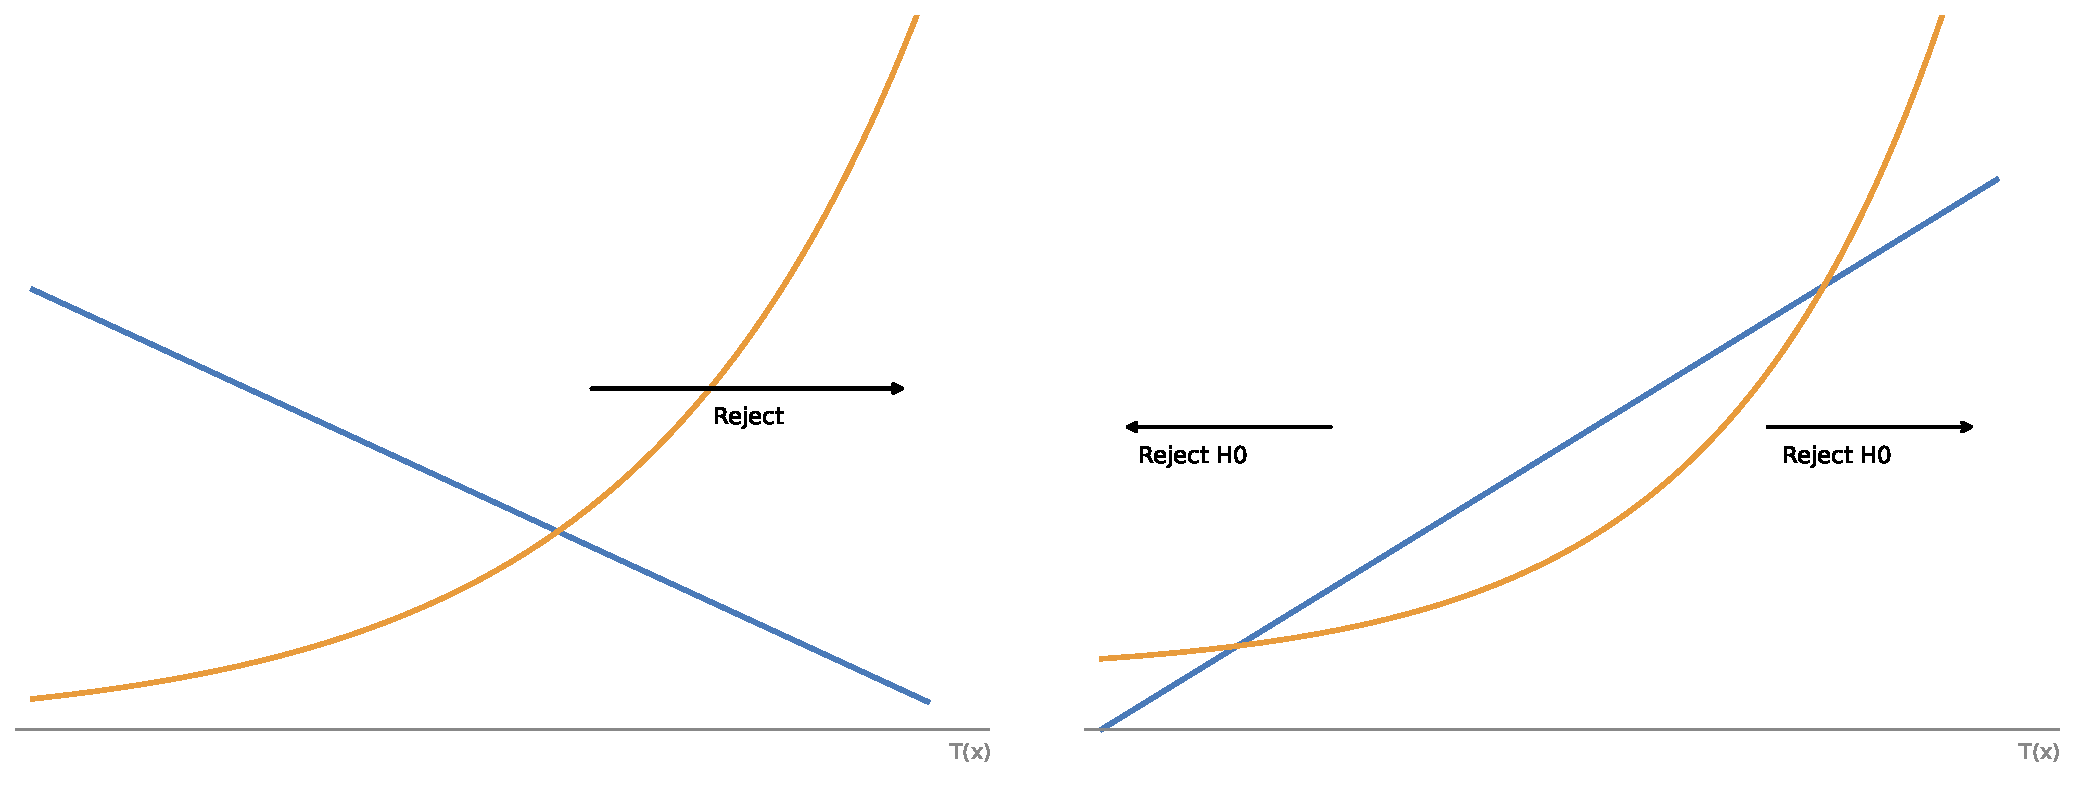
\includegraphics[width=0.9\linewidth]{figures/rejection_regions.pdf}
    \caption{Rejection Regions}
    \label{fig:rejection_regions}
\end{figure}


The first possibility will not give rise to an unbiased test, because the result would be a one-sided test with monotone power functions. Therefore any optimal $\phi$ is of the form
\[
\phi(x) = \begin{cases} 1 & \text{if } T(x) > C_1 \text{ or } T(x) < C_2 \\ \gamma_i & \text{if } T(x) = C_i \\ 0 & \text{otherwise} \end{cases}.
\]
A simplification is possible if $T(x)$ is symmetrically distributed under $\theta_0$. Then the optimal test rejects whenever $|T(x)| > \text{const}$. Such tests are called \textbf{equitailed tests}.

\subsubsection{UMP Invariant Tests}
\begin{exam}
Suppose that we observe $X = (X_1, \ldots, X_d)$, with independent coordinates $X_i \sim \mathcal{N}(\theta_i, 1)$ and that we are interested in the hypothesis testing problem
\[
H_0 : \theta_1 = \ldots = \theta_d = 0 \quad \text{vs.} \quad H_1 : \exists i \in \{1, \ldots, d\} : \theta_i \neq 0.
\]
If we transform our data so that $X' = OX$ for $O \in \mathbb{O}(d)$, the set of $d \times d$ orthogonal matrices, i.e., the set of square matrices such that $O^\top O = OO^\top = I$, then we have $X_i' \stackrel{\text{ind}}{\sim} \mathcal{N}(\theta_i', 1)$ for $\theta' = O\theta$, and our hypothesis testing problem can be seen to be equivalent to testing
\[
H_0 : \theta_1' = \ldots = \theta_d' = 0 \quad \text{vs.} \quad H_1 : \exists i \in \{1, \ldots, d\} : \theta_i' \neq 0.
\]
Hence, when searching for a test, the \textbf{principle of invariance} would suggest constraining $\phi(X) = \phi(OX) \; \forall O \in \mathbb{O}(d)$. In this case, it can be checked that $\phi$ is invariant in this way iff it is a function of the magnitude of the vector of samples, i.e.\ of $T = \sum_i X_i^2$. This tells us that if we only care about invariant tests, our optimality goal is to search for UMP tests among functions of $T$.

In this example, $T$ is non-central chi-squared distributed with $d$ degrees of freedom, i.e., $T \sim \chi_d^2(\psi^2)$ with a non-centrality parameter $\psi^2 = \sum_{i=1}^{d} \theta_i^2$. Thus, we can simplify the null and alternative hypotheses of our testing problem to
\[
H_0 : \psi = 0 \quad \text{vs.} \quad H_1 : \psi > 0. \quad \text{(one-sided test)}
\]
Note that we have reduced both the relevant data and the relevant parameter space for our testing problem; these are common advantages of imposing invariance constraints. To derive our UMP invariant test, we will check that the $\chi_d^2(\psi^2)$ has monotone likelihood ratios in $T$. Note that the density of non-central chi-squared distribution has the form:
\[
f(t; \psi) = e^{-\frac{\psi^2}{2}} \sum_{k=0}^{\infty} \frac{\left(\frac{\psi^2}{2}\right)^k}{k!} \cdot \frac{t^{\frac{d}{2} - 1 + k} e^{-\frac{t}{2}}}{2^{k + \frac{d}{2}} \Gamma\left(k + \frac{d}{2}\right)}.
\]
The likelihood ratio can therefore be computed as
\[
\frac{p_{\psi^2}(t)}{p_{\psi^2 = 0}(t)} = \frac{f(t; \psi)}{\frac{t^{\frac{d}{2} - 1} e^{-t/2}}{2^{\frac{d}{2}} \Gamma\left(\frac{d}{2}\right)}} = e^{-\frac{\psi^2}{2}} \sum_k c_k \left(\frac{\psi^2}{2}\right)^k t^k.
\]
where $c_k$ are non-negative constants. We can see that each term in the sum above increases in $t$, and thus the ratio as a whole is increasing in $t$. (We only need to compare each parameter value with $0$, because our null hypothesis is simple.) Thus this family has MLR, and the UMPI test rejects when $T$ is large.
\end{exam}

\subsubsection{Confidence Regions}
\begin{defn}[Confidence region]
A set $S(X)$ satisfying $\mathbb{P}_\theta[\theta \in S(X)] \ge 1 - \alpha$, for all 
$\theta \in \Omega$ is known as a $1 - \alpha$ \textbf{confidence region}, with a 
$1 - \alpha$ \textbf{confidence level}.
\end{defn}
Given a model $\mathcal{P} = \{\mathbb{P}_\theta : \theta \in \Omega\}$, we begin 
by defining an appropriate collection of tests. For each $\theta_0 \in \Omega$, let 
$\Omega_0(\theta_0)$ be a set containing $\theta_0$, where 
$\Omega_0(\theta_0) \subset \Omega$. Next, define $\phi_{\theta_0}$ to be a level 
$\alpha$ test for $H_0: \theta \in \Omega_0(\theta_0)$ vs.\ 
$H_1: \theta \notin \Omega_0(\theta_0)$, and define $A(\theta_0)$ as the acceptance 
region of $\phi_{\theta_0}$. Because $\phi_{\theta_0}$ is a level 
$\alpha$ test, and $\theta_0 \in \Omega_0(\theta_0)$, we have 
$P_\theta(X \in A(\theta)) \ge 1 - \alpha$ for all $\theta \in \Omega$.

Now consider the region $S(X) = \{\theta \in \Omega : X \in A(\theta)\}$. Since 
$P_\theta(\theta \in S(X)) = P_\theta(X \in A(\theta)) \ge 1 - \alpha$, $S(X)$ is a 
$1 - \alpha$ confidence region! Different choices of null sets $\Omega_0(\theta_0)$ 
will lead to different forms of confidence regions. For example,
\begin{enumerate}
  \item \textbf{One-sided tests} $\Omega_0(\theta_0) = \{\theta : \theta \le \theta_0\}$ 
  often yield \textbf{confidence bounds}
  \[
    S(X) = \{\theta : u(X) \le \theta\}
  \]
  where $u(X)$ denotes a data-dependent lower bound.
  \item \textbf{Two-sided tests} $\Omega_0(\theta_0) = \{\theta_0\}$ often yield 
  \textbf{confidence intervals}
  \[
    S(X) = \{\theta : u(X) \le \theta \le v(X)\},
  \]
  where $v(X)$ denotes a data-dependent upper bound.
\end{enumerate}

Intuitively, we desire a $1 - \alpha$ confidence region that is as narrow as 
possible, which we can achieve by minimizing the number of extraneous it contains. 
We make this notion precise in the following optimality property for confidence 
regions.

\begin{defn}[UMA]
A $1 - \alpha$ confidence region $S(X)$ is \textbf{uniformly most accurate} if, 
among all $1 - \alpha$ regions, $\mathbb{P}_\theta(\theta' \in S(X)) 
= \mathbb{P}_\theta(X \in A(\theta'))$ is minimized for all $(\theta, \theta')$ 
satisfying $\theta \notin \Omega_0(\theta')$.
\end{defn}

\subsection{Multiple Testing and Error Rate Control}

\subsubsection{Bonferroni’s Test and Fisher's Test}
We focus on global testing first with a number of null hypotheses $H_{0,i}$. We may care about the global null hypothesis
\[
H_0 = \bigcap_{i=1}^n H_{0,i}.
\]
We’ll assume that our p-values have the super-uniform property that (here $p_i$ is a random variable coming out of the test)
\[
\PP (p_i\le t) = t
\]
under the null hypothesis.

\begin{defn}[Bonferroni's Global Test]
Let $\alpha$ be some desired significance level (for example $0.05$), and suppose we have $n$ different hypotheses. \textbf{Bonferroni's global test} rejects the global null if
\[
\min_i p_i \leq \frac{\alpha}{n}.
\]
\end{defn}

\begin{prop}[Size of Bonferroni's Global Test]
If the $p$-values are super-uniform then Bonferroni's procedure has \textbf{size} (that is, chance of Type I error) at most $\alpha$.
\end{prop}

\begin{proof}
The probability of rejecting the null under the null hypothesis is, by a union bound and the super-uniform property
\begin{align*}
\mathbb{P}(\text{reject}) &= \mathbb{P}\left(\bigcup_{i=1}^{n} \left\{p_i \leq \frac{\alpha}{n}\right\}\right) \\
&\leq \sum_{i=1}^{n} \mathbb{P}\left(p_i \leq \frac{\alpha}{n}\right) \\
&\leq n \cdot \frac{\alpha}{n} \\
&= \alpha.
\end{align*}
\end{proof}
\begin{rem}
    Notice that this does not require any independence assumptions, and in fact if we assume p-values are uniform and independent then 
    \begin{align*}
    \mathbb{P}(\text{reject}) &=1- \mathbb{P}\left(\bigcap_{i=1}^{n} \left\{p_i \geq \frac{\alpha}{n}\right\}\right) \\
    &= 1-\left(1 - \frac{\alpha}{n}\right)^n \\
    &\approx 1- e^{-\alpha} \\
    &\approx \alpha - \frac{\alpha^2}{2} +\cdots.
    \end{align*}
\end{rem}
\begin{rem}
    But if we’re not under the global null, we will not “hug the uniform line $y=x$” anymore – sometimes (1) these sorted p-values will have a few that are extremely small and then the rest generally following the line (meaning maybe five hypotheses have very strong signals), and sometimes (2) all of the p-values will be overall deflated (too small). Bonferroni’s method is really most useful in case (1), because it will successfully reject due to the very small p-values; it will not reject the null in case (2) and thus is not a very powerful test.
\end{rem}
\begin{defn}[Fisher's Combination Test]
\textbf{Fisher's combination test} rejects the global null using a more combined measure. Specifically, we consider the test statistic
\[
T = -\sum_{i=1}^{n} 2 \log p_i,
\]
and we reject the null if $T$ is large.
\end{defn}
\begin{prop}
Assume that $p_1, \cdots, p_n$ are \textbf{independent} and uniform (for example in meta-analysis, suppose we do not have overlapping patients among the studies). Then under the null hypothesis, we have $T \sim \chi^2_{2n}$ (that is, the chi-square distribution with $2n$ degrees of freedom).
\end{prop}
Now we need to discuss which test is better. Consider a particular ``needle in a haystack" problem. 
Let $Y_i \sim N(\mu_i, 1)$ independently for $i = 1, \ldots, n$, and consider the global null
\[
H_0 : \mu_1 = \cdots = \mu_n = 0 \quad \text{vs.} \quad H_1 : \exists\, i,\ \mu_i \neq 0.
\]
Under $H_0$, Bonferroni's statistic $\max_i Y_i$ concentrates around $\sqrt{2 \log n}$. So we have power only when some $\mu_i > \sqrt{2 \log n}$ — the ``needle in a haystack'' threshold. Plotting power against $\mu_i / \sqrt{2 \log n}$, there is a sharp phase transition at $1$: power is $\approx \alpha$ below and $\approx 1$ above.

Assume the size of ``needle" $h = \sqrt{2r\log n}$. We will prove no $\alpha$-level test with some nontrivial power for $r=1-\epsilon$. The point is to avoid having a composite alternative: instead, consider the Bayesian decision problem with null hypothesis
\[
H_0 : \mu_i = 0 \text{ for all } i
\]
and a ``simple'' alternative hypothesis
\[
H_1 : \{\mu_i\} \sim \pi,
\]
where $\pi$ selects a coordinate uniformly at random and sets its mean to $\mu^{(n)}$, keeping all other means to zero.

The most powerful test in such a setting where $H_0, H_1$ are both simple hypotheses is the likelihood ratio test, and if we can show it has no power then everything else will have no power. Indeed, we have likelihoods
\[
f_0(y) = \prod_{j=1}^{n} \frac{1}{\sqrt{2\pi}} \exp\left(-\frac{1}{2} y_j^2\right), \quad f_1(y) = \frac{1}{n} \sum_{i=1}^{n} \frac{1}{\sqrt{2\pi}} \exp\left(-\frac{1}{2}(y_i - \mu)^2\right) \prod_{j : j \neq i} \frac{1}{\sqrt{2\pi}} \exp\left(-\frac{1}{2} y_j^2\right).
\]
and we want to reject when $\frac{f_1}{f_0}$ is large. What's nice is that all the terms cancel out except the shifted mean:
\[
L = \frac{1}{n} \sum_{i=1}^{n} \exp\left(Y_i \mu - \frac{1}{2} \mu^2\right).
\]
Notice that this is different from Bonferroni — it's a softmax instead of looking at the maximum, since if $\mu = \infty$ this would be completely dominated by the maximum $Y_i$. This is nice because it's just a sum of iid terms of mean $1$, and in fact if $\mu$ is small enough this likelihood concentrates:

\begin{prop}
Under the null hypothesis, if $\mu^{(n)} = (1 - \epsilon)\sqrt{2 \log n}$, then $L \to 1$ in probability as $n \to \infty$.
\end{prop}
Under such proposition, if we set threshold $T_n(\alpha)$ so that $\PP_{\HH_0}(L\ge T_n(\alpha)) = \alpha$, then
\begin{align*}
\mathbb{P}(\text{type II error}) = \mathbb{P}_{H_1}(L \leq T_n(\alpha)) &= \int \mathbf{1}\{L \leq T_n(\alpha)\} \, dP_{H_1} \\
&= \int L \cdot \mathbf{1}\{L \leq T_n(\alpha)\} \, dP_{H_0} \\
&= \int \mathbf{1}\{L \leq T_n(\alpha)\} \, dP_{H_0} + \int (L - 1) \mathbf{1}\{L \leq T_n(\alpha)\} \, dP_{H_0} \\
&\to (1-\alpha) + 0,
\end{align*}
\[
\implies \mathbb{P}(\text{type I error})+\mathbb{P}(\text{type II error}) \to 1.
\]
\begin{rem}
    Consider Fisher's combination test with
    \[
    T = \sum_{i=1}^n Y_i^2 = \|\bY\|_2^2.
    \]
    By CLT, we have
    \[
    \frac{T- (n+\|\mu\|_2^2)}{\sqrt{2n+4\|\mu\|_2^2}} \sim \mc N(0,1).
    \]
    And the test is powerful when $\|\mu\| > \sqrt{2n}$ and us quite large compared to something like Bonferroni. In slightly different terminology, the main parameter that mattered here was proportional to the signal-to-noise ratio
    \[
    \text{SNR} = \frac{\text{signal power}}{\text{expected noise power}} = \frac{\|\mu\|^2}{\sigma^2 n}
    \]
\end{rem}
Our original model was that we had independent statistics $X_i$ which are $N(0, 1)$ under the null hypothesis and $N(\mu_i, 1)$ under the alternative, but now we want to extend to a setting where we have a small fraction of non-null hypotheses. Thus we will now use a simple model where
\[
H_0 : X_i \stackrel{\text{iid}}{\sim} N(0, 1), \quad H_1 : X_i \stackrel{\text{iid}}{\sim} (1 - \varepsilon) N(0, 1) + \varepsilon N(\mu, 1).
\]
In the literature we historically parameterize
\[
\varepsilon_n = n^{-\beta}, \quad \frac{1}{2} < \beta < 1,
\]
\[
\mu_n = \sqrt{2r \log n}, \quad 0 < r < 1.
\]
It turns out that we have a threshold curve
\[
\rho^*(\beta) = \begin{cases} \beta - \frac{1}{2} & \frac{1}{2} < \beta \leq \frac{3}{4}, \\ (1 - \sqrt{1 - \beta})^2 & \frac{3}{4} \leq \beta \leq 1, \end{cases}
\]
such that Neyman-Pearson has full power for $r > \rho^*(\beta)$ (that is, we can adjust the test so that the sum of type I and type II error probabilities approaches $0$) and no power for $r < \rho^*(\beta)$ (that is, for any test, the limiting sum of type I and type II error is at least $1$). A crude calculation, we get power if
\[
\max_{\text{non-null}} X_i \approx \sqrt{2r \log n} + \sqrt{2 \log n^{1-\beta}} > \sqrt{2 \log n}.
\]

\subsubsection{Higher Criticism}
In general, the whole point is that in global testing we do not know $\epsilon$ and $\mu$ and thus cannot use the NP test in the first place. We introduce Tukey’s higher criticism.
\[
HC_n^* = \max_{0 < \alpha \leq \alpha_0} \frac{F_n(\alpha) - \alpha}{\sqrt{\alpha(1 - \alpha)/n}}.
\]
\begin{rem}
    The process $\sqrt{n}(F_n(t) - t)$ will converge in distribution to a Brownian bridge, and the maximum of this rescaled Brownian bridge on $(1/n, \alpha_0)$ converges in probability to $\sqrt{2 \log \log n}$ (this is the law of the iterated logarithm). 
    And a result of Donoho and Jin says that rejecting when $HC_n^* \geq \sqrt{(1 + \varepsilon) 2 \log \log n}$ gives us $\mathbb{P}_0(\text{type I}) + \mathbb{P}_1(\text{type II}) \to 0$ for any $r$ above the detection threshold.
\end{rem}

\begin{rem}
    The main problem is that near $t = 0$, we are no longer approximately normal --- $B(n, p)$ is nicely approximated by a Gaussian if $np$ is not too small, but if $np$ is small we get something that's Poisson, which has much heavier tails. The Burk-Jones statistic is an attempt to resolve this problem, but it is not fully effective.
    The idea is that for each $t$, we can test whether $n\hat{F}_n(t) < t$ using a likelihood ratio test
    \[
    \log LR_n(t) = \begin{cases} nD(\hat{F}_n(t), t) & 0 \leq t \leq F_n(t), \\ 0 & \text{otherwise}, \end{cases}
    \]
    where $D(p_0, p_1) = p_0 \log \frac{p_0}{p_1} + q_0 \log \frac{q_0}{q_1}$, $q_i = 1 - p_i$ is the Kullback-Leibler divergence. We then define
    \[
    BJ^+ = \max_{1 \leq i \leq n/2} nD\left(p_{(i)}, \frac{i}{n}\right)
    \]
    that is, at what significance level we detect a divergence between what we see and what we expect.
\end{rem}

\subsubsection{False Discovery Rate}
We now turn to identifying which hypotheses are non-null and to controlling the false discovery rate.
\begin{table}[h]
\centering
\begin{tabular}{c|cc|c}
 & accepted & rejected & total \\
\hline
true  & $U$ & $V$ & $n_0$ \\
false & $T$ & $S$ & $n - n_0$ \\
\hline
total & $n - R$ & $R$ & $n$ \\
\end{tabular}
\end{table}

\begin{defn}[Familywise Error Rate]
The \textbf{familywise error rate (FWER)} is defined to be $\mathbb{P}(V \geq 1)$.
\end{defn}

\begin{thm}[Bonferroni's Method]
Bonferroni's method controls FWER at level $\alpha$; more specifically, if there are $n_0 \leq n$ null hypotheses, we get
\[
\mathrm{FWER} \leq \mathbb{E}[V] = \frac{n_0}{n}\alpha.
\]
\end{thm}

\begin{proof}
Since $V$ is nonnegative-integer-valued, we have $\mathbb{P}(V \geq 1) \leq \mathbb{E}[V]$. And letting $\mathcal{N}_0$ denote the set of null hypotheses, we have
\[
\mathbb{E}[V] = \mathbb{E}\left[\sum_{i \in \mathcal{N}_0} \mathbf{1}\left\{p_i \leq \frac{\alpha}{n}\right\}\right] = \sum_{i \in \mathcal{N}_0} \mathbb{P}\left(p_i \leq \frac{\alpha}{n}\right) = n_0 \cdot \frac{\alpha}{n},
\]
which completes the proof.
\end{proof}

Suppose we have $n$ hypotheses $H_{(1)}, \ldots, H_{(n)}$ corresponding to the \textbf{ordered} $p$-values $p_{(1)} \leq \cdots \leq p_{(n)}$ (so we choose $H_{(1)}$ to be the hypotheses with the most surprising $p$-value, and so on). Now we will compare $p$-values with an adaptive threshold based on what we've seen so far.

What we do here is called a \textbf{Holm's procedure procedure}:
\begin{itemize}
    \item First, compare with Bonferroni's threshold: if $p_{(1)} \leq \frac{\alpha}{n}$, then reject $H_{(1)}$ and move to the next step. Otherwise, reject nothing (accept all null hypotheses).
    \item Now in general for step $i$, if $p_{(i)} \leq \frac{\alpha}{n - i + 1}$, then reject $H_{(i)}$ and go to the next step ($i + 1$). Otherwise, accept \underline{$H_{(i)}, H_{(i+1)}, \ldots, H_{(n)}$} and stop.
    \item Finally, if $p_{(n)} \leq \alpha$, then we reject $H_{(n)}$; otherwise we accept it.
\end{itemize}
Notice that
\[
\{V \geq 1\} = \{\text{procedure reached } i_0\} \cap \left\{p_{(i_0)} \leq \frac{\alpha}{n - i_0 + 1}\right\},
\]
and $\mathbb{P}(V \geq 1) \leq \alpha$.

However, FWER is so stringent that we often return nothing if we require FWER control.
\begin{defn}[False Discovery Proportion \& False Discovery Rate]
The \textbf{false discovery proportion (FDP)} is given by
\[
\mathrm{FDP} = \frac{V}{\max(R, 1)} = 
\begin{cases}
V/R & R \geq 1 \\
0 & \text{otherwise}
\end{cases}
\]
(this last case is just by convention so that we can control this quantity). In general this random variable is unobserved, and the \textbf{false discovery rate (FDR)} is the expectation $\mathrm{FDR} = \mathbb{E}[\mathrm{FDP}]$ of this quantity.
\end{defn}

We'll now consider a procedure generally more powerful than Holm's procedure -- instead of Hochberg's procedure, we consider a step-up procedure with critical values $\alpha_i = \frac{\alpha i}{n}$, which is far less conservative than $\frac{\alpha}{n - i + 1}$.

\begin{thm}[Controlling FDR]
Suppose our test statistics are independent (so $p$-values are independent). Then the Benjamini-Hochberg controls the FDR at level $\alpha$. More precisely, we actually have the expression
\[
\mathrm{FDR} = \frac{n_0}{n}\alpha \leq \alpha.
\]
\end{thm}

\begin{proof}
Let $V_i = \{H_i \text{ rejected}\}$ be the indicator function for hypothesis $i$ being rejected. By definition, we have
\[
\mathrm{FDP} = \sum_{i \in \mathcal{H}_0} \frac{V_i}{R \vee 1}.
\]
Now, it suffices to show that for any null $i$, we have $\mathbb{E}\left[\frac{V_i}{R \vee 1}\right] = \frac{\alpha}{n}$. (This is somehow ``the only answer we can get'' because the nulls are uniform and thus the random variables are exchangeable.) To prove this claim, notice that we can do casework over the value of $R$ and write
\[
\frac{V_i}{R \vee 1} = \sum_{k=1}^{n} \frac{V_i \mathbf{1}\{R = k\}}{k} = \sum_{k=1}^{n} \frac{\mathbf{1}\left\{p_i \leq \frac{\alpha k}{n}\right\} \mathbf{1}\{R = k\}}{k},
\]
since assuming $R = k$, we know the threshold for rejection is $\frac{\alpha k}{n}$. Notice that on the event $p_i \leq \frac{\alpha k}{n}$, changing $p_i$ to zero doesn't change the threshold, meaning whenever we reject $H_i$, the number (and identity) of rejections is the same. So we can write the above expression as
\[
\sum_{k=1}^{n} \frac{\mathbf{1}\left\{p_i \leq \frac{\alpha k}{n}\right\} \mathbf{1}\{R(p_i \to 0) = k\}}{k},
\]
where this notation means that we set this null $p$-value to zero. Now we can take the expectation of this quantity conditioned on all other $p$-values -- the only randomness is in $p_i$ here, so
\begin{align*}
\mathbb{E}\left[\frac{V_i}{R \vee 1} \,\bigg|\, p_1, \ldots, p_{i-1}, p_{i+1}, \ldots, p_n\right] 
&= \sum_{k=1}^{n} \frac{\frac{\alpha k}{n} \mathbf{1}\{R(p_i \to 0) = k\}}{k} \\
&= \sum_{k=1}^{n} \frac{\alpha}{n} \mathbf{1}\{R(p_i \to 0) = k\} \\
&= \frac{\alpha}{n}.
\end{align*}
Then finally taking the expectation over the last $p$-value yields the result.
\end{proof}

Consider dependency,
\begin{thm}[Guo-Rao '08]
Let $S(n) = 1 + \frac{1}{2} + \cdots + \frac{1}{n} \approx \log n + 0.577$ be the $n$th harmonic number. Then there are joint distributions where the FDR of the Benjamini-Hochberg procedure $BH(\alpha)$ is at least $\min(1, \alpha S(n))$.
\end{thm}

\begin{thm}[Benjamini-Yekutieli '01]
Under dependence of $p$-values, the $BH(\alpha)$ procedure does control at level $\alpha S(n)$; in fact,
\[
\mathrm{FDR} \leq \alpha S(n) \cdot \frac{n_0}{n}.
\]
\end{thm}

The following proof is also by Professor Cand\'es and a former student:

\begin{proof}
Let $\alpha_i = \frac{i\alpha}{n}$; much like in the proof before, it suffices to show that $\mathbb{E}\left[\frac{V_i}{R \vee 1}\right] = \frac{\alpha}{n} S(n)$. We again have
\[
\frac{V_i}{R \vee 1} = \sum_{k=1}^{n} \frac{\mathbf{1}\{p_i \leq \alpha_k\} \mathbf{1}\{R = k\}}{k},
\]
and we look at where $p_i$ can fall. Summing over the possible ranks it can take on, we have
\[
\sum_{k=1}^{n} \sum_{\ell=1}^{k} \frac{\mathbf{1}\{\alpha_{\ell-1} \leq p_i \leq \alpha_\ell\} \mathbf{1}\{R = k\}}{k} = \sum_{\ell=1}^{k} \sum_{k \geq \ell} \frac{\mathbf{1}\{\alpha_{\ell-1} \leq p_i \leq \alpha_\ell\} \mathbf{1}\{R = k\}}{k}
\]
just by swapping the order of summation. But now if we do the $k$-sum first, we're just looking at the probability of getting a particularly high number of rejections, so this simplifies to
\[
\sum_{\ell=1}^{n} \frac{\mathbf{1}\{R \geq \ell\}}{R} \mathbf{1}\{p_i \in [\alpha_{\ell-1}, \alpha_\ell]\}.
\]
Everything so far has been an equality, so ``nothing interesting'' has happened yet. But now we can simplify the first fraction to be bounded by $\frac{1}{\ell}$,
\[
\sum_{\ell=1}^{n} \frac{1}{\ell} \mathbf{1}\{p_i \in [\alpha_{\ell-1}, \alpha_\ell]\} = \sum_{\ell=1}^{n} \frac{1}{\ell} \frac{\alpha}{n} = S(n) \frac{\alpha}{n},
\]
and then the rest of the proof proceeds as before. What's surprising is that the result of Guo and Rao shows that there are distributions of $p$-values for which this inequality is indeed tight!
\end{proof}

\subsubsection{E-Values}
\begin{exam}
Consider the following situation (which is real): research group $A$ tests a medication and gets a promising but not conclusive result (whatever that means -- perhaps it's risky to go to trial). Then research group $B$ tests again on new data, but it's still not clear, so research group $C$ tests next (again on new data). We then want to understand how to combine these test results together even when we aren't following a fixed plan.
\end{exam}
Another bad news is in many cases we can not get p-values easily.
The e-value is a generic replacement of the p-value which will handle this problem of optional continuation.

\begin{defn}
Recall that a null hypothesis $\mathcal{H}_0$ is basically a collection of probability measures. An \emph{$e$-variable $E$ for testing $\mathcal{H}_0$} is a nonnegative random variable such that
$$\sup_{P_0 \in \mathcal{H}_0} \mathbb{E}_{P_0}[E] \leq 1.$$
A realization of an $e$-variable is called an \emph{$e$-value}. Meanwhile, a \emph{$p$-variable for testing $\mathcal{H}_0$} is a nonnegative random variable that satisfies
$$\sup_{P_0 \in \mathcal{H}_0} \mathbb{P}_{P_0}(P \leq \alpha) \leq \alpha$$
for all $\alpha \in (0,1)$, and a realized value of a $p$-variable is a $p$-value.
\end{defn}

\begin{prop}
For any $e$-value $E$, the random variable $E^{-1}$ is a conservative $p$-value (meaning that it is a $p$-value with wiggle room).
\end{prop}
\begin{proof}
Indeed, we have
$$\mathbb{P}\left(\frac{1}{E} \leq \alpha\right) = \mathbb{P}\left(E \geq \frac{1}{\alpha}\right) \leq \frac{\mathbb{E}[E]}{1/\alpha} \leq \alpha.$$
\end{proof}

\begin{exam}
We'll be looking at \textbf{safety under optional continuation} in this lecture: suppose $(X_1, Z_1), (X_2, Z_2), \ldots$ is our data, where $Z_i$ is some ``side information'' (for example, whether we have enough money to keep running experiments). Suppose that the data comes in batches of size $n_1, n_2, \ldots$, and $N_t = \sum_{i=1}^{t} n_i$ is the size of the data we have so far.
\end{exam}

We'll establish an $e$-value $E_1$ on the first batch. From there, we evaluate an $e$-value $E_2$ on the next batch, but only if the outcome is in a certain range (promising but not conclusive) and the external factors take on certain values (things that we cannot plan) -- otherwise we stop early. Then depending on the outcomes and external factors up until the second batch, we decide whether or not to compute $E_3$, and so on. But the point is that after $\tau$ total data batches, \textbf{the final result we report is the product}
\[
V_\tau = \prod_{i=1}^{\tau} E_i.
\]
In particular, we're allowed to choose whether to continue on depending on whether each individual $E_i$ is above some threshold of our choice, and the point is that we'll still be able to control the type I error:

\begin{thm}
Regardless of the stop-continue rule, as long as $\tau$ is a stopping time, $V_\tau$ is itself an $e$-value. More formally, let $\mathcal{F}_t$ be a filtration. Suppose that for all $t$, the conditional $e$-variable $E_t$ is a nonnegative random variable which is $\mathcal{F}_t$-measurable, and such that for all $P_0 \in \mathcal{H}_0$ we have $\mathbb{E}_{P_0}[E_t | \mathcal{F}_{t-1}] = 1$. (This is easy to check in practice.) Then $V_t = \prod_{i \leq t} E_i$ is a nonnegative supermartingale under the null. Thus by the optional stopping theorem, for any stopping time $\tau$ with respect to the filtration, $V_\tau = \prod_{t=1}^{\tau} E_t$ is an $e$-value. (In particular, $V_t$ is an $e$-value for each fixed $t$.)
\end{thm}

Now we focus on multiple testing.
\begin{defn}
In the \textbf{e-BH procedure}, we reject the hypotheses of the largest $\hat{k}$ e-values, where
\[
\hat{k} = \max\left\{i : \frac{i e_{(i)}}{n} \geq \frac{1}{\alpha}\right\}.
\]
\end{defn}

\begin{rem}
We should be careful that $\frac{1}{p}$ is not an $e$-value in general (in fact its expectation need not be finite), even though $\frac{1}{e}$ is always a $p$-value.
\end{rem}

\begin{thm}[Wang--Ramdas '20]
The $e$-BH procedure has FDR at most $\frac{n_0 \alpha}{n}$, and no independence assumption is required.
\end{thm}

\subsection{Causal Inference}
\subsubsection{Randomized Controlled Trials}
A traditional view holds that statistics is concerned with inferring correlations or associations among variables. From this perspective, causal inference appears to have no place in statistics. In this section, however, we will discuss several statistical methods for estimating causal effects in both randomized experiments and observational studies.

We define the causal effect of a treatment via potential outcomes. For a binary treatment $w \in \{0, 1\}$, we define potential outcomes $Y_i(1)$ and $Y_i(0)$ corresponding to the outcome the $i$-th subject would have experienced had they respectively received the treatment or not. The \textbf{causal effect of the treatment on the $i$-th unit} is then
\[
    \Delta_i = Y_i(1) - Y_i(0).
\]
The fundamental problem in causal inference is that only one treatment can be assigned to a given individual, and so only one of $Y_i(0)$ and $Y_i(1)$ can ever be observed. Thus, $\Delta_i$ can never be observed.
Now, although $\Delta_i$ itself is fundamentally unknowable, we can (perhaps remarkably) use \textbf{randomized experiments} to learn certain properties of the $\Delta_i$. In particular, large randomized experiments let us recover the average treatment effect (ATE)
\[
    \tau = \mathbb{E}\left[Y_i(1) - Y_i(0)\right].
\]

\textit{}When an RCT is unavailable, we can use observational data  $(X_i,Y_i,W_i)$ to construct an estimator for the ATE. 
Considering the \textbf{propensity score}
\[
e(x) = \mathbb{P}\left[W_i = 1 \mid X_i = x\right],
\]
and we construct the inverse-propensity weighting estimator
\[
\hat{\tau}_{IPW} = \frac{1}{n} \sum_{i=1}^{n} \left( \frac{W_i Y_i}{\hat{e}(X_i)} - \frac{(1 - W_i) Y_i}{1 - \hat{e}(X_i)} \right).
\]
\begin{rem}
    IPW relies on the unconfoundedness assumption
    \[
    \{Y_i(0), Y_i(1)\} \indep W_i \mid e(X_i).
    \]
    Many real-world policies assign treatment by a sharp rule on a running variable (e.g., scholarships above a GPA cutoff). Units just above and below the cutoff are nearly identical in all other respects, so the discontinuity creates a local "as-if randomized" experiment.
\end{rem}



\subsection{Conformal prediction}
\subsubsection{Fundamentals}
Suppose $X_1, \ldots, X_n$ are iid samples from some probability distribution $P$, and $Y_1, \ldots, Y_m$ are iid samples from some other probability distribution $Q$. Our goal is to test the hypothesis that $P = Q$ even if we don't know either of the distributions.
The strategy we learn in early statistics is that we should choose a test statistic $T$ (for example we can let $T = |\overline{X} - \overline{Y}|$) and reject the null based on whether $T$ is unusually large. The question we need to ask is ``how large does $T$ need to be,'' and typically this is where permutation tests are introduced: we compare $T$ to how the statistic would look \textbf{if we were to permute the data}.

Formally, we introduce the following (randomized) \textbf{permutation distribution}: choose $M$ uniform permutations $\sigma_1, \ldots, \sigma_M$ from $S_{n+m}$ (the set of permutations acting on a list of $n + m$ objects), and we will have these permutations act on the vector
\[
Z = (X_1, \ldots, X_n, Y_1, \ldots, Y_m).
\]
Specifically, the $\sigma_i$s will shuffle the entries of $Z$, and then we evaluate the test statistic on the permuted entry. So we always take the average of the first $n$ entries and the average of the last $m$ entries after permuting, and we find their absolute difference; in other words, we compare
\[
T(Z) = \left|\overline{Z_{1:n}} - \overline{Z_{n+1:n+m}}\right|
\]
to the corresponding values of $T(Z_\sigma)$, and the $p$-value will essentially be the relative rank of $T(Z)$ compared to $T(Z_{\sigma_1})$ through $T(Z_{\sigma_M})$:
\[
p = \frac{1 + \sum_{i=1}^{M} \mathbf{1}\{T(Z_{\sigma_i}) \geq T(Z)\}}{1 + M}.
\]
Under the null, this is either uniformly distributed on $\left\{\frac{1}{M+1}, \frac{2}{M+1}, \ldots, \frac{M+1}{M+1}\right\}$ or biased upward due to ties (because under the null we have exchangeability of the vector $Z$). Thus it is indeed a $p$-value, and notice that this doesn't rely on us needing to know the distribution of $T$ at all.
Given a set of permutations $S$, consider the quantity
\[
p = \frac{1 + \sum_{\sigma \in S} \mathbf{1}\{T(Z_\sigma) \geq T(Z)\}}{1 + |S|}.
\]
If the variables are exchangeable, then $Z_\sigma$ has the same distribution as $Z$ and thus $T(Z_\sigma)$ has the same distribution as $T(Z)$. We are interested in what sets of permutations $S$ yield a valid $p$-value.
Here are the answers:
\begin{center}
\begin{tabular}{c|c}
$S$ & $p$-value? \\
\hline
all permutations ($S_n$) & Yes \\
iid samples from $S_n$ & Yes \\
an arbitrary fixed subset of $S_n$ & No \\
iid samples from an arbitrary fixed subset & No \\
a subgroup of $S_n$ & Yes \\
iid samples from a subgroup of $S_n$ & Yes \\
\end{tabular}
\end{center}

\begin{exam}[Conformal Prediction]
In predictive inference, we take some set of training samples $(X_1, Y_1), \ldots, (X_n, Y_n)$ which are iid from some distribution $P$. We then get a test sample $X_{n+1}$, and our goal is to construct, from the training samples, a prediction interval for $Y_{n+1}$ with prescribed coverage. That is, we want some $C$ so that
\[
\mathbb{P}(Y_{n+1} \in C(X_{n+1})) \geq 1 - \alpha.
\]
\end{exam}

Note that this is not a confidence interval -- this is an observation we have not seen yet, and it's interesting that we can solve this problem at all. In fact, the way we can do so is through permutation tests! We hypothesize a value of $Y_{n+1}$ and test for exchangeability by computing
\[
p^y = \frac{1}{(n+1)!} \sum_{\sigma \in S_{n+1}} \mathbf{1}\{T(Z^y_\sigma) \geq T(Z^y)\},
\]
where $Z^y = \{(X_1, Y_1), \ldots, (X_n, Y_n), (X_{n+1}, y)\}$. Then setting $y \in C(X_{n+1})$ if and only if $p^y \geq \alpha$, we claim this is a valid prediction interval regardless of our choice of $T$. Indeed, $Y_{n+1}$ itself will be in the confidence interval if and only if $p^{Y_{n+1}} \geq \alpha$, but we've already shown that $p^{Y_{n+1}} \stackrel{\text{sto}}{\geq} U$ and thus we are done.

The motivation for conformal prediction is that we want some uncertainty in our prediction and some way of quantifying accuracy.

\subsubsection{Approaches}
\textbf{Full conformal prediction}  is typically done as follows: we fit a model $\hat{\mu}(\cdot) = \mathcal{A}(Z^y)$ to $Z^y = ((X_1, Y_1), \ldots, (X_n, Y_n), (X_{n+1}, y))$ which satisfies the symmetry assumption (for example in random forests, it doesn't matter what order we pass in the data, and this is true of most algorithms), and we define $T(Z^y) = |y - \hat{\mu}(X_{n+1})|$ to be the residual. Replacing $T$ with what we have, we thus get a $p$-value
\[
p^y = \frac{1}{n+1} \sum_{i=1}^{n+1} \mathbf{1}\{|Y_i - \hat{\mu}(X_i)| \geq |y - \hat{\mu}(X_{n+1})|\} = \frac{1}{n+1} \sum_{i=1}^{n+1} \mathbf{1}\{R^y_i \geq R^y_{n+1}\}.
\]
and again we include $y$ in the interval if and only if $p^y\ge \alpha$. This is all computationally intensive – every time we fit the model we might need to do a lot of computation, and in fact the prediction interval can be a disjoint set of intervals instead.

We introduce \textbf{split conformal prediction} then. This is a special case where we have $n$ data points and we do sample splitting: we learn a model $\hat{\mu}$ with the first split (also called a ``fold''), and on the second split we calculate out-of-sample residuals (that is, learn the distribution of the residuals $R_i = |Y_i - \hat{\mu}(X_i)|$). Then the test residual relates to this second split by keeping track of quantiles, and the point is that we separately do training and calibration and form our interval from points that have all not been used for training.

Formally, we compute a score function $S(x, y) = |y - \hat{\mu}(x)|$ by fitting a model on an independent training set. Once we have this, we use a distinct calibration set of size $n$ to find typical size of residuals
\[
S_i = S(X_i, Y_i), \quad S^y_{n+1} = S(X_{n+1}, y).
\]
The point is that if $y = Y_{n+1}$ these points should all be indistinguishable (they're from the same distribution), and now we include $y$ if
\[
p^y = \frac{1}{n+1} \sum_{i=1}^{n} \mathbf{1}\{S_i \geq S^y_{n+1}\} \geq \alpha.
\]
And this result now holds conditionally on the training set, since for all purposes $\hat{\mu}$ is fixed.

\begin{rem}
    Other methods to estimate $\hat{\mu}$ include Leave-One-Out and Cross-Validation.
\end{rem}


\subsection{Application: Watermark Detection}
\todo